\documentclass{standalone}
\usepackage{tikz}

\begin{document}
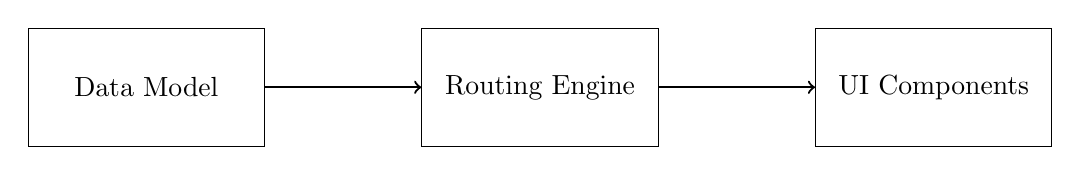
\begin{tikzpicture}

% Define boxes
\node[draw, rectangle, minimum width=3cm, minimum height=1.5cm] (box1) at (0, 0) {Data Model};
\node[draw, rectangle, minimum width=3cm, minimum height=1.5cm] (box2) at (5, 0) {Routing Engine};
\node[draw, rectangle, minimum width=3cm, minimum height=1.5cm] (box3) at (10, 0) {UI Components};

% Draw arrows
\draw[->, thick] (box1.east) -- (box2.west);
\draw[->, thick] (box2.east) -- (box3.west);

\end{tikzpicture}
\end{document}